\section{Evaluation}
\label{cha:evaluation}

We evaluate our design by first implementing it, then running the experiment using it and concluding with analysing the results of the experiment.

\subsection{Implementation}
\label{sec:implementation}

\subsubsection{Dataset Generator}
We have decided to not use an off the shelf dataset or dataset generator like BerlinMOD \cite{duntgenBerlinMODBenchmarkMoving2009}, but to implement our own generator.

We developed a data generator simulating e-scooter trips in Berlin using Python 3.\footnote{\url{github.com/erykksc/escooter-trips-generator}}
We used the OpenStreetMap data through OSMnx library to extract the biking network, points of interest and administrative boundaries (in the rest of the thesis we refer to them as localities).

Inside the repository we also define a flake.nix file, which allows us to match the exact versions of Python interpreter and all the libraries used using nix, ensuring repeatability and reproducibility of the dataset generation.
Additionally we use a seed value in order for the pseudo random generators to yield the same dataset each run.

Using the generator we simulate 1 billion trips from 01-01-2020 to 31-12-2025.
The generator create trips in a following manner:
\begin{enumerate}
	\item Start point and start time of every trip are chosen randomly from uniform distributions seen on \cref{fig:trip-start-point-distribution} and \cref{fig:trip-time-distribution}
	\item A random bearing is chosen, also from a uniform distribution seen on \cref{fig:trip-bearing-distribution}
\item The route traverses through nodes in a direction of a random bearing, choosing nodes with the smallest bearing difference to our chosen bearing.
	We extend the route by adding nodes to it until we reach the threshold length defined by a Log-normal distribution with $\alpha=0.5$, scale=2100 (median ~2100m) seen on \cref{fig:trip-route-length-distribution}.
\item We model the speed between the nodes along the trip with a Beta distribution with $\alpha=8, \beta=1$ scaled to 0-20 km/h, seen on \cref{fig:trip-speed-distribution}.
	We chose this distribution as 20km/h is max legal speed in Germany and a driver needs to slow down on turns or traffic lights but tends to ride close to the max speed.
\item Using the speed and the distance between the nodes, the time to travel between the nodes is computed.
\item Using the route, start time, and time to travel between individual nodes of the route, we create a single trip.
	A trip consist of many events. 
	An event is a single data entry with following fields and types:
	\begin{itemize}
		\item \textbf{event\_id} - UUIDv4
		\item \textbf{trip\_id} - UUIDv4
		\item \textbf{timestamp} - ISO 8601 timestamp with timezone offset
		\item \textbf{latitude} - float
		\item \textbf{longitude} - float
	\end{itemize}
\end{enumerate}

\begin{figure}
    \begin{subfigure}{0.49\linewidth}
        \centering
        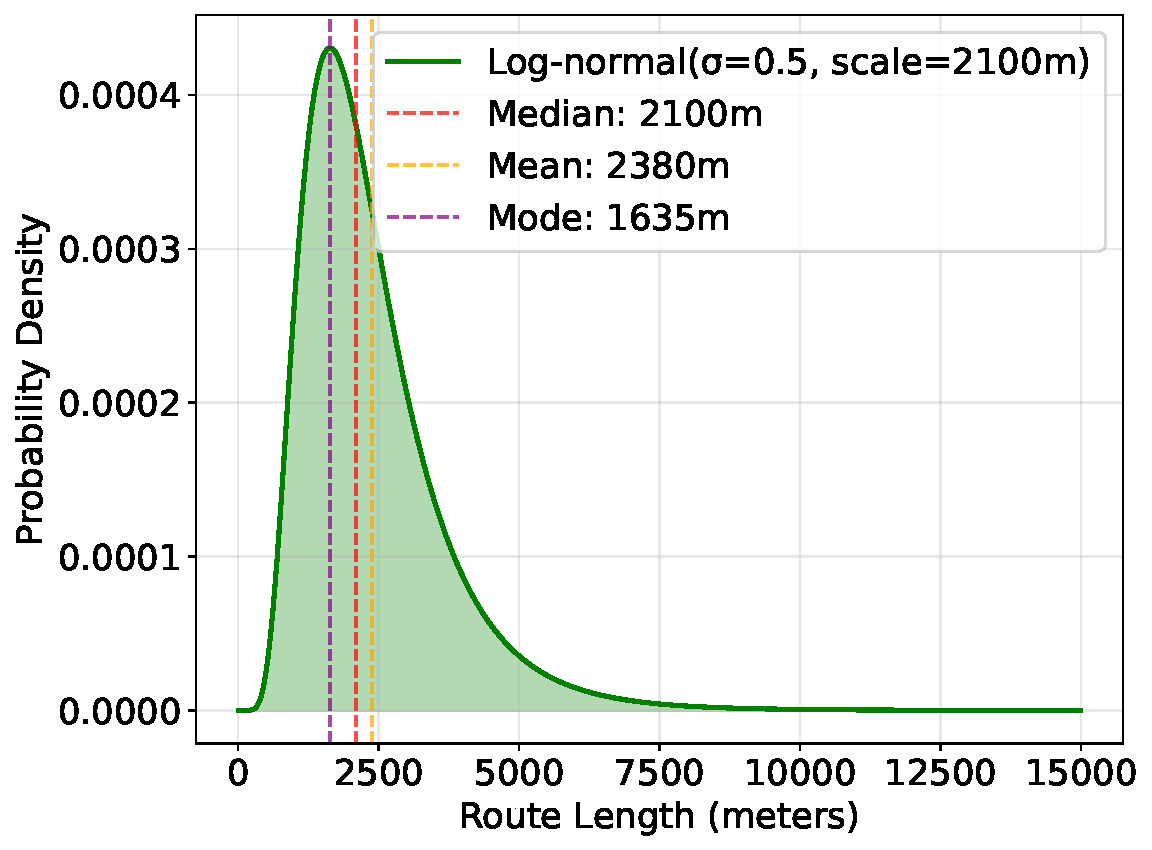
\includegraphics[width=\linewidth]{./fig/route-length-distribution-no-labels.pdf}
        \caption{Route length distribution}
        \label{fig:trip-route-length-distribution}
    \end{subfigure}
    \hfill
    \begin{subfigure}{0.49\linewidth}
        \centering
        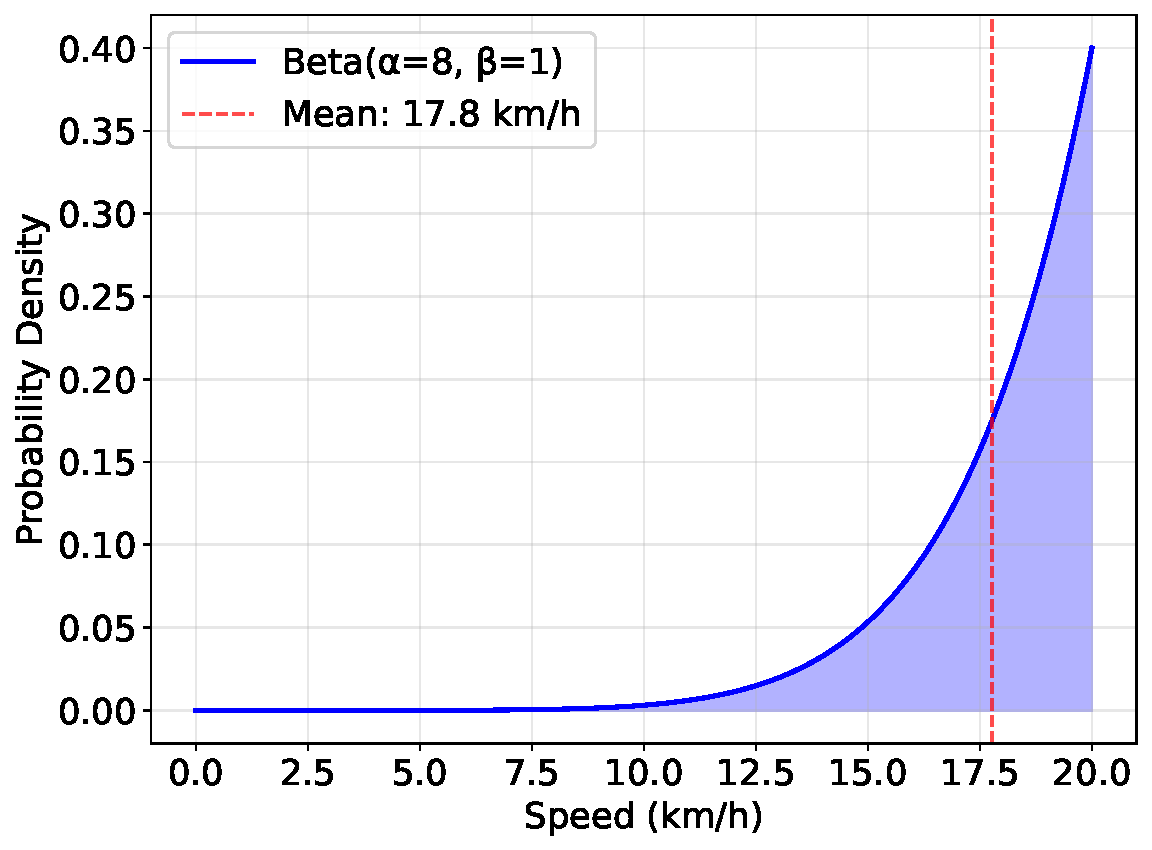
\includegraphics[width=\linewidth]{./fig/speed-distribution-no-labels.pdf}
        \caption{Escooter speed distribution}
        \label{fig:trip-speed-distribution}
    \end{subfigure}
    \vfill
    \begin{subfigure}{0.49\linewidth}
        \centering
        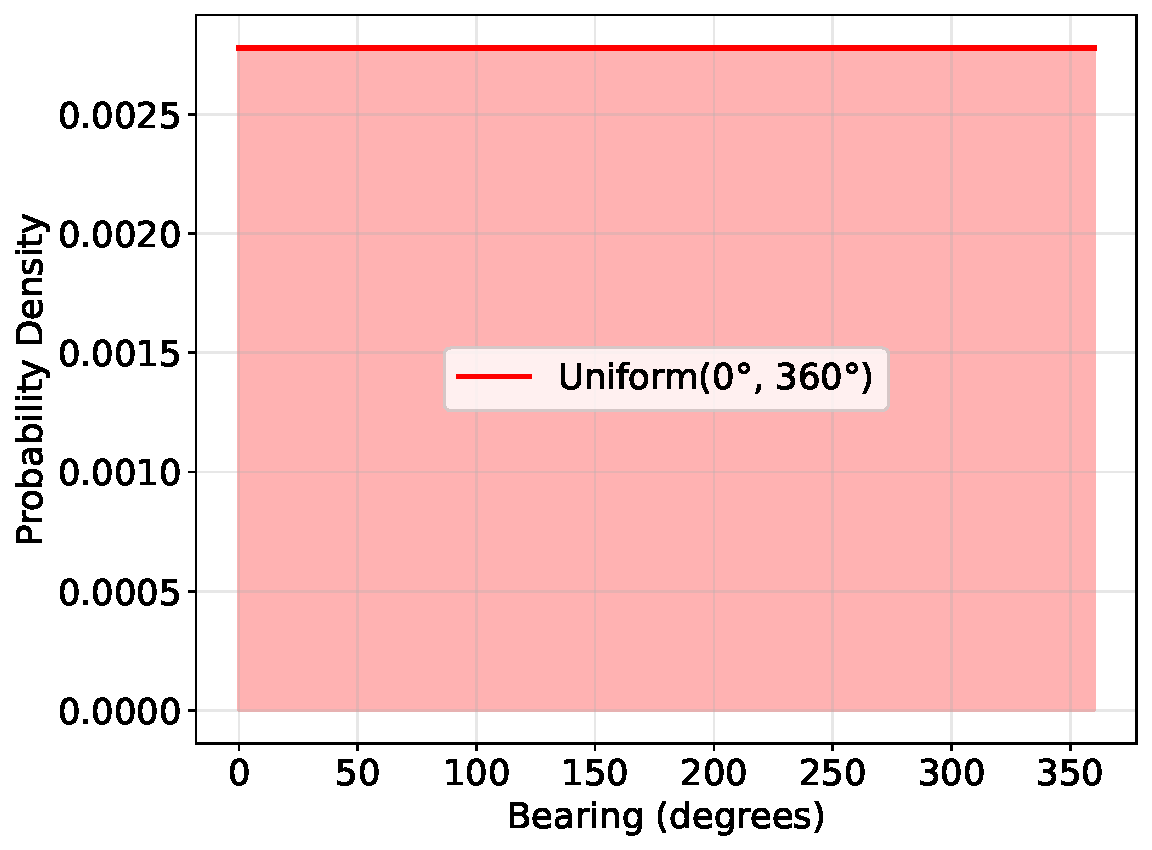
\includegraphics[width=\linewidth]{./fig/bearing-distribution-no-labels.pdf}
        \caption{Bearing of a trip distribution}
        \label{fig:trip-bearing-distribution}
    \end{subfigure}
    \hfill
    \begin{subfigure}{0.49\linewidth}
        \centering
        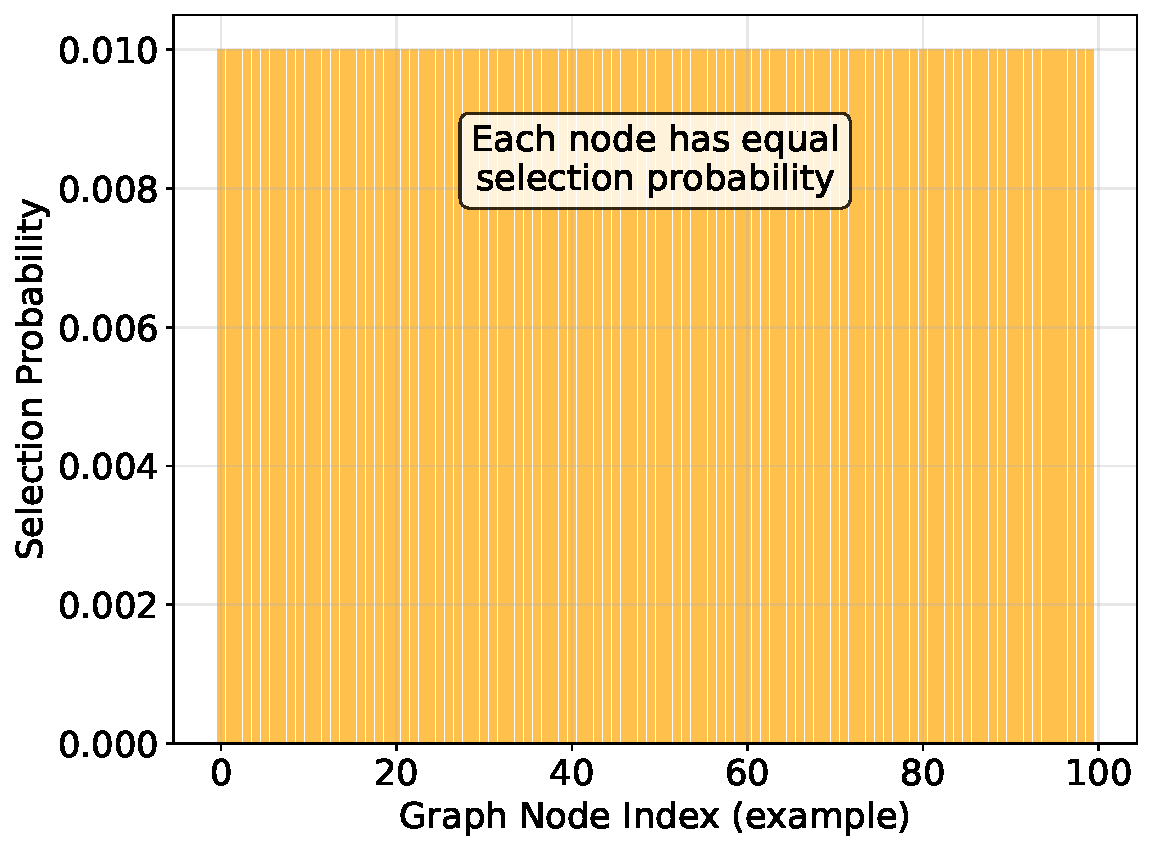
\includegraphics[width=\linewidth]{./fig/start-point-distribution-no-labels.pdf}
        \caption{Start point of a trip distribution}
        \label{fig:trip-start-point-distribution}
    \end{subfigure}
    \vfill
    \begin{subfigure}{0.49\linewidth}
        \centering
        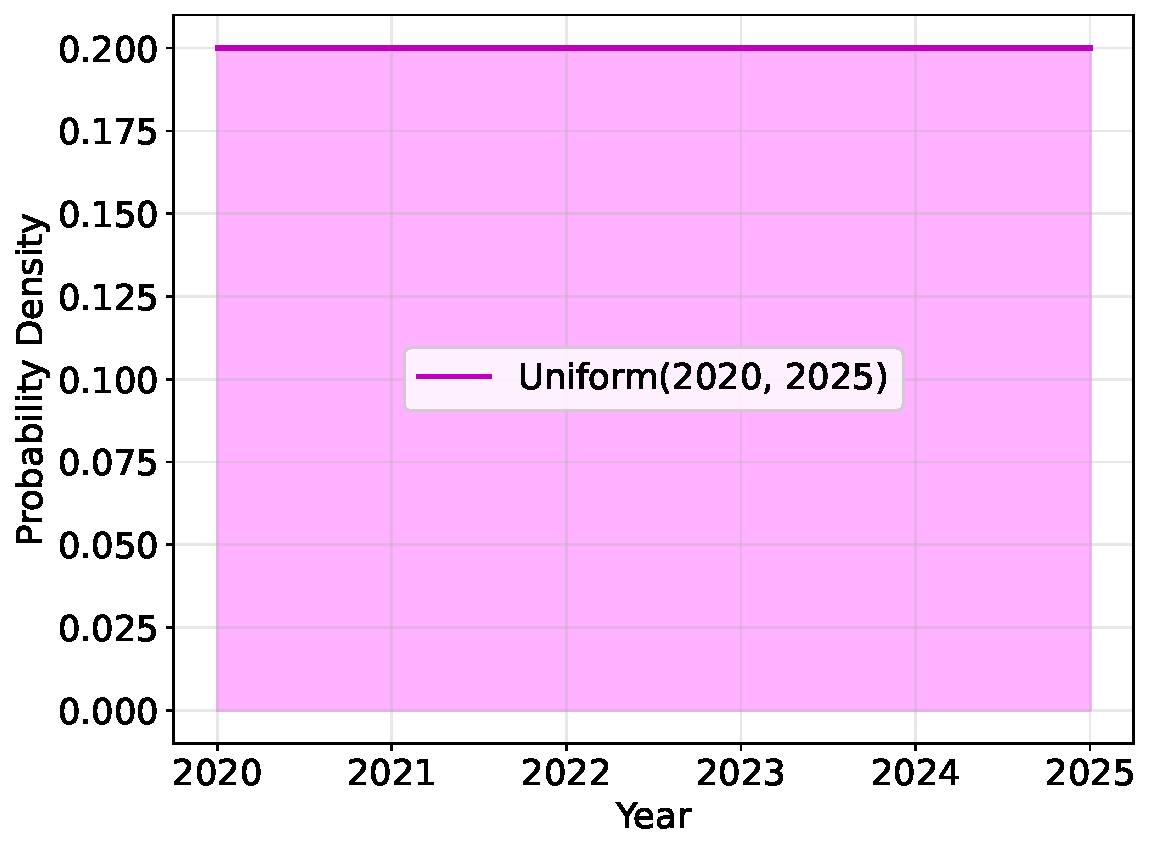
\includegraphics[width=\linewidth]{./fig/time-distribution-no-labels.pdf}
        \caption{Start time of a trip distribution}
        \label{fig:trip-time-distribution}
    \end{subfigure}
    \caption{Distributions we used in our dataset generator for simulating e-scooter trips}
    \label{fig:generator-distributions}
\end{figure}

We saved the simulated trips into a CSV file for our load-generator to consume.

\subsubsection{Load-Generator}
We implement the load-generator in Go (version 1.24).
We choose this programming language due to its builtin concurrency features: 
(1) go-routines - lightweight, user-space threads managed by the Go runtime, and
(2) channels - allow safely communication between go-routines.

We made this decision to simulate many simultaneous DDBMS clients, each consuming little memory.
Goroutines are resource-efficient as the Go runtime performs the N:M mapping of goroutines to OS threads.\footnote{\url{https://go.dev/src/runtime/HACKING}}
This way we can scale to thousands or even millions of concurrent clients on a single machine, as each client is primarily I/O-bound.

Next, we implement 3 modes to the load-generator to run the 3 scenarios from the design:
\begin{enumerate}
	\item \textbf{initialize} - initializes tables and indexes
	\item \textbf{insert} - inserts e-scooter events into DDBMS, implementing the insert scenario
	\item \textbf{query} - queries DDBMS using randomized queries from a file with templates.
		We implement two template files for each DDBMS, one containing the simple queries and the second one implementing the complex queries.
\end{enumerate}


\subsubsection{Insert Queries}
We insert the e-scooter events from the generated CSV file into DDBMS using multiple concurrent connections.

The insert process works on a basis of a work queue, a pattern described by Burns and Oppenheimer \cite{196346} i.e., main thread reads data from the CSV file and adds jobs to the queue.
The workers read the jobs containing the events data from the queue and execute insert queries on the DDBMS while collecting metrics.

The queue is implemented using go-channel avoiding race conditions and manual mutex locks as the go-channels provide built-in synchronization.
Individual worker threads measure the metrics from the DDBMS alongside the time they have spent waiting for their next job (ideally, wait time for next job should be 0).
We have added this mechanism in order to ensure that the speed at which main thread reads from file is not a bottleneck as this would make load-generator a bottleneck in the benchmark.

We implemented two modes of inserts into load-generator: batch and bulk.
In the batch mode we insert multiple single SQL queries into a single request, reducing the network trips.
We made the batch size configurable so it is possible to send single insert queries.
On the other hand, in the bulk we send single request with a configurable amount of events.

\subsubsection{Read Queries}

We split the read queries into two categories, simple and complex.
By doing that we want to simulate two user categories (1) clients (2) analysts.

Consequently, the simple queries, the ones simulating individual clients, consist of queries that query for information about a single trip.
We have identified 8 queries relevant for an e-scooter user:
\begin{enumerate}
	\item \textbf{Length of a trip} - retrieve the length of a specific trip (e.g., in the summary after a trip)
	\item \textbf{Trip events} - retrieve all events of a trip (e.g., in order to display them on a map)
	\item \textbf{Average speed of a trip} - retrieve average speed during the trip (e.g., in the summary after a trip)
	\item \textbf{Trip start locality} - retrieve the locality the trip started in (i.e., part of the city where the trip started)
	\item \textbf{Trip finish locality} - retrieve the locality the trip ended in (i.e., part of the city where the trip ended)
	\item \textbf{First and last location of a trip} - retrieve the first and last location of a trip (e.g., in order to show simplified summary view on a map)
	\item \textbf{POIs close to the finish location} - retrieve points of interest in a specific radius around the finish location (e.g., in order to show shops nearby)
	\item \textbf{POIs within radius during the trip} - retrieve which points of interests the user has driven past through during his trip (e.g., in order to mark certain touristic attractions as visited)
\end{enumerate}

After the simple queries, we define 7 complex queries.
Those queries aim to mimic the queries an analyst may sent to DMBS in order to gain insight into traffic, find possible optimization points.
In order to imitate that we defined the following queries, each of them queries about a specific time frame:
\begin{enumerate}
	\item \textbf{Trips in locality} - Which trips have passed through a specified locality in time frame
	\item \textbf{Most visited POIs} - which points of interests had trips that were in specified distance from them in a specified time frame
	\item \textbf{N closest trips to POI} - find n trips that came the closest to a point of interest in a specified time frame
	\item \textbf{Average trip duration per locality} - calculate the average trip duration per locality in a specified time frame
	\item \textbf{Start and end in different localities} - how many trips started and ended in different locality in a specified time frame
	\item \textbf{Event density heat-map per locality} - generate heat-map of e-scooter usage by area and hour
	\item \textbf{Trips summaries} - summaries about trips in time frame e.g., minimal, maximal, average of length, duration of a trip as well as of the event count for trips
\end{enumerate}

% TODO: add the section that mobilitydb is inspired from the tutorial and then the cratedb has been 
% created to mimic this functionality. There were
The queries are inspired by the online tutorial [FOOTNOTE LINK], but have been adapted fo

All the queries are parametrized so they do not repeat.
We generate the actual queries on the fly inside the load-generator during execution. 
The random generator is set to a seed and we use a work queue pattern, same as in the insert mode.
As the seed is set based on the query number and base seed, allowing reproducibility of every query.
We choose a query template in a rotating fashion, so that the each subsequent template is different from the past one.
This ensures that we will not be biased towards one DDBMS by generating different queries for it.

\subsubsection{Infrastructure}
We implemented the infrastructure as code using OpenTofu, an open source terraform fork.\footnote{\url{https://opentofu.org/}}
Using it we defined three deployments:
\begin{enumerate}
	\item \textbf{Shared} - defines shared infrastructure between load-generator and AKS-cluster i.e., subnet, virtual network, and a resource group
	\item \textbf{Load-Generator} - defines the virtual machine (VM) used as load-generator
	\item \textbf{AKS Cluster} - defines Kubernetes cluster running on Azure Kubernetes Service (AKS)
\end{enumerate}

Using three deployments allows us to take down the Kubernetes cluster without affecting the load-generator VM.
This is important as the load-generator stays the same between benchmark runs and the size of the AKS-cluster changes.

\subsubsection{DDBMS Deployment}

We have decided to use containerization in order to improve portability and allow easy local development.
We automated the deployment by choosing Kubernetes as the container orchestration tool.
We chose it over Docker swarm as it has wider adoption, thus improving relevancy as it is more likely that DDBMS will be deployed this way.

We used the provided official Kubernetes operator to deploy the CrateDB clusters.

For the MobilityDBC there was no official nor unofficial docker image, so we developed our own.\footnote{\url{https://github.com/erykksc/citus-mobilitydb}}
We used PostgreSQL 17 image as base for the image as it is the newest supported version by Citus at time of writing.\footnote{\url{https://www.citusdata.com/updates/v13-0/}}
As the PostgreSQL 17 image is based on Debian, we used the official instructions from Citus webpage on top of PostgreSQL.\footnote{\url{https://www.citusdata.com/download}} to install Citus 13 (newest at time of writing)
The installation of Citus required adding additional repository to Debian's package manager APT, while MobilityDB package was in the official repositories.
We automatically enable the Citus, MobilityDB, and PostGIS (dependency of MobilityDB) on the container startup.
We published the image to GitHub Container Registry (GHCR) under MIT License.

Individual worker nodes of MobilityDBC need to be manually connected to the coordinator node, as Citus doesn't support auto discovery.
For this job, we developed a Manager, a Docker container which when added to the Kubernetes cluster with right permissions, automatically detects new pods running Citus and connects them to the Coordinator.
We also published the images to GHCR under MIT License.\footnote{\url{https://github.com/erykksc/citus-k8s-manager}}
CrateDB clusters do not require such manager as the nodes support auto discovery and elect the master node themselves.\footnote{\url{https://cratedb.com/docs/guide/admin/clustering/multi-node-setup.html}}
We created two Helm charts in order to simplify the deployment of the DDBMS, one for CrateDB and one for MobilityDB.
\footnote{\url{[GITHUB REPO URL]}}
Using Helm charts we are able to deploy a collection of Kubernetes deployments such as stateful sets with the nodes, internal and external services, storage classes required to run DDBMS.
We choose Helm charts as they allow parametrization using templating, so change of Storage Class or number of nodes in cluster can be changed using a CLI argument.
Kubernetes by itself does not support this feature and relies on external tools, such as Helm.

\subsection{Experiment Results}
\label{sec:experiment-results}

% \subsection{Load-Generator}
% This approach allows easy data collection, compared to using multiple load-generators running on multiple hosts and makes the benchmark cheaper to run.
% We believe this strategy is viable, as the load-generator primarily issues requests, which are i/o heavy, so the performance of the computer running the software shouldn't be a bottleneck.
% % * this benchmark load-generator is placed on the same VPC in the cloud as the cluster with running DDBMS
% The load-generator is also put on the cloud in the same virtual private cloud (VPC) as the DDBMS cluster.
% Putting the load-generator next to the SUT instead of running it on our local computer allows us to minimize latency and potential disturbances while the benchmark runs i.e., packages dropped due to network problems.


% \subsection{DDBMS cluster}
% We document the DDBMS cluster configuration through Kubernetes deployment files ensuring that the software will be deployed with the same settings and versions using versioned container images.
% Additionally by using Kubernetes, the benchmark can also be more easily developed on local systems by using contenerization.
% The local development has been an important consideration as the recent withdrawal of Google from issuing cloud tokens to our university, lead to uncertainty to where the benchmark will be deployed.
% Kubernetes has been chosen over using bash scripts for installing DDBMS on multiple virtual machines for two reasons.
% (1) It allows easier deployment of a DDBMS cluster, which is beneficial when deploying multiple cluster sizes and resetting their state by destroying them.
% (2) Relevancy, as deployment of such clustered DDBMS systems is often done this way in production environments (CITATION HERE)

% In the benchmark the load-generator will connect with the System Under Test (SUT) and issue queries.
% It will log metrics allowing later analysis of the findings.
% The System Under Test, will be run on the same resources i.e., MobilityDB will be deployed on the same resources as CrateDB.
% The resources for the SUT will be restarted between each benchmark run to ensure a clean state.

% \subsection{Design Objectives}
% The benchmark should be relevant to real-world use cases, especially spatial-temporal workloads as this is the primary value proposition of MobilityDB over other databases.
% We accomplish that by modelling queries after common use cases like, time slice queries, window queries, and spatiotemporal joins.
% We deploy the SUTs on a Kubernetes cluster in Microsoft Azure, resembling common deployment method of companies.
% Such deployment using infrastructure as code, allows us to share the configuration of SUTs, as well as information of provisioned cloud resources, allowing reproducibility of our results.

% The decision to choose Kubernetes over shell scripts or other automation tools such as Ansible has reduced understandability (as not everybody is familiar with container orchestration tools such as Kubernetes), but allowed us to improve portability, relevance and simplified development.
% This trade off has been made as unexpectedly because of the cloud infrastructure provider, where we wanted to run the benchmark on initially, cut off credits for the university right before the start of the thesis writing.
% Such change, made us switch to a solution that was more portable.
% Using containerization, allowed us to develop on single host machine without creating VMs and also made it possible to run our benchmark on other cloud providers or university servers/Kubernetes cluster.
% Furthermore, use of containers improves repeatability as the node will have exact same versions of the software installed on them.

% The SUTs are benchmarked using equivalent conditions ensuring fairness by
% (1) deploying them on the same cloud resources (processor types, memory, storage, and networking),
% (2) running semantically analogous queries,
% (3) connecting same amount of clients to them, and by
% (3) inserting same amount of data.
% Notably, \mobilitydbc~supports more complex queries than CrateDB and because of that we will benchmark queries supported by both systems.
% We suspect that \mobilitydbc~ being full ACID compliant will result in reduced raw performance, but in this thesis we focus on scalability patterns so are making this trade-off to fairness.

% Our benchmark evaluates scalability by measuring how each SUT performs under growing cluster sizes and data volumes.

% We decided to benchmark the following sizes for the SUT clusters, 2, 3, 4, and 5.
% Preferably we would benchmark the DDBMS on larger cluster sizes to improve relevance of our findings, but due to resource constrain we choose to do it on a set of small ones to reduce costs.
% Despite the small difference in size between the sizes, we hope to see a pattern which would allow us to create conclusions about scalability.

% To check how well the databases handle multiple simultaneous connections and try to find a pattern, we have decided to benchmark the SUT on following number of simultaneous clients 100, 1000, 10000.

% % \subsection{Kubernetes explanation}
% %
% % Important aspect of this benchmark was the portability as there was uncertainty where would the experiment be conducted.
% % Three environments had to be taken into account.
% % First, the cloud, initially it was planned to run the experiment on Google Cloud Platform but unfortunately, Google suddenly stopped providing credits for the University.
% % Two, the server cluster of the University, with support for Kubernetes.
% % Our machines, for testing and in case it wouldn't be possible to use different computers.
% %
% % Ultimately we have decided to go with Kubernetes, as it provided a way to run the database systems on all of the three environments, as well as increasing the benchmark relevance, as we assume the production systems are likely gonna be deployed in such environment.
% % Additionally use of Kubernetes increased ease of use, as it is a common solution for distributed systems, along with robustness, as Kubernetes automatically revives dead nodes, allows to easily change replica count and extend the configuration for real life systems.
% %
% % For the data used for the benchmark we decided to use a synthetic data generator that would be run as a pod on the same Kubernetes cluster in order to minimize possible, latency and unknown variables on the network.
% \subsection{Quality Metrics}
% % TODO: Move this entire section to Evaluation chapter - metrics definitions, percentile breakdowns, IoT relevance justification
% To measure scalability we plot the Metric curves over increasing node counts.
% We choose the following metrics for our benchmark
% (1) Latency, it will be measured in milliseconds for both inserts and queries. We will create percentile breakdown (P50,P95, P99) to provide insight into tail latencies.
% (2) Throughput, we will measure the number of records written or queries completed per second.

% In the context of IoT devices, write throughput is important for the devices themselves, and the read latency is important for the users.
% Because of this, the benchmark results should be relevant.

% \subsection{Workload design}
% % TODO: Move to separate "Workload Design" chapter or merge into Evaluation. Move Go implementation details to Implementation chapter.
% We adopt a synthetic workload combined with a micro-benchmark approach where each run isolates one quality of system behavior (e.g., write latency, read throughput).
% This avoids confounding metrics and ensures interpretable results. We have developed a custom synthetic workload-generator, written in Golang, which will issue concurrent requests using lightweight goroutines to simulate a fixed large number of clients.
% Golang has been chosen due to goroutines, which are lightweight threads (~2KB stack vs ~1MB stack when using OS threads) managed by the Go runtime, allowing us to simulate a large number of concurrent clients on a relatively small system.

% For the write workload we will simulate IoT devices emitting time-stamped spatial data of %TODO: what will the generated data be of?
% We will test batch and single-record inserts at varying ingestion rates to measure write throughput and latency.

% Whereas for the read workload, we will simulate %TODO: what will we simulate exactly?
% This will be performed by running following queries
% (1) Temporal range queries (e.g., last hour of data per device).
% (2) Spatial bounding box queries (e.g., devices within a bounding box).
% (3) Spatio-temporal window queries (e.g., average speed over 10-minute intervals).

% \subsection{Measurement}
% % TODO: Move this entire section to Evaluation chapter - measurement methodology, goroutine details, resource monitoring specifics
% We combined the load-generator with the testing client in order for the same goroutine to issues requests as well as to measure their metrics.
% This way we keep the measuring simple and understandable and don't overcomplicate the setup.

% In order to minimize unknown variables, such as network latency, reliability, and interference of other devices, we put the load-generator on the same Kubernetes cluster.
% The load-generator pod runs on a separate Kubernetes node, a different host machine, isolated from database nodes to prevent influencing SUT performance.
% During the evaluation we monitor the resource usage of every node, focusing on the load-generator in order to prevent it from becoming a bottleneck in the benchmark.
